\section{Конструкторский раздел}

В данном разделе описываются требования к разрабатываемому методу и программному комплексу, реализующему интерфейс для метода. Рассматривается архитектура метода и структура программного комплекса.

\subsection{Требования к разрабатываемому методу}

Метод распознавания челюстно--лицевых костей черепа по томографическим снимкам головы человека (далее --- метод распознавания) должен:
\begin{itemize}
	\item Принимать на вход изображения в форматах PNG, JPG, JPEG.
	\item Производить семантическую сегментацию зубочелюстных костей и костей челюстно--лицевого сустава.
	\item Производить сегментацию экземпляров распознанных зубов.
\end{itemize}

\subsection{Требования к разрабатываемому программному комплексу}

Программный комплекс, реализующий интерфейс для разработанного метода, должен предоставлять:
\begin{itemize}
	\item Возможность загрузки изображений через графический интерфейс.
	\item Возможность выбора этапов работы: сегментация зубочелюстного сустава или челюстно--лицевого, семантическая сегментация или сегментация экземпляров.
	\item Создание итогового снимка с выделенными сегментированными зонами.
\end{itemize}

\subsection{Проектирование метода разспознавания}

В качестве основы для метода распознавания будет применяться нейронная сеть UNet.

UNet при обучении использует готовые маски, поэтому необходимо будет произвести предварительную разметку данных для выделения масок костей зубочелюстного и черепно--лицевого суставов.

После обучения при работе модели UNet составляет маску области, по которой происходит дальнейшее выделение объектов. Для сегментации зубов по экземплярам стоит на данном этапе составить вектора особенностей для каждого зуба, что поможет произвести классификацию по типу.

\subsubsection{Физиология зубочелюстного сустава}

Существует четыре типа зубов:
\begin{itemize}
	\item Резцы --- служат для захвата и откусывания пищи.
	\item Клыки --- необходимы для разрывания и удерживания пищи.
	\item Премоляры --- раздавливают и передавливают пищу.
	\item Моляры --- измельчают и перемалывают пищу.
\end{itemize}

На рисунке \ref{fig:teeth} представлена классификация зубов.

\begin{figure}[H]
	\centering
	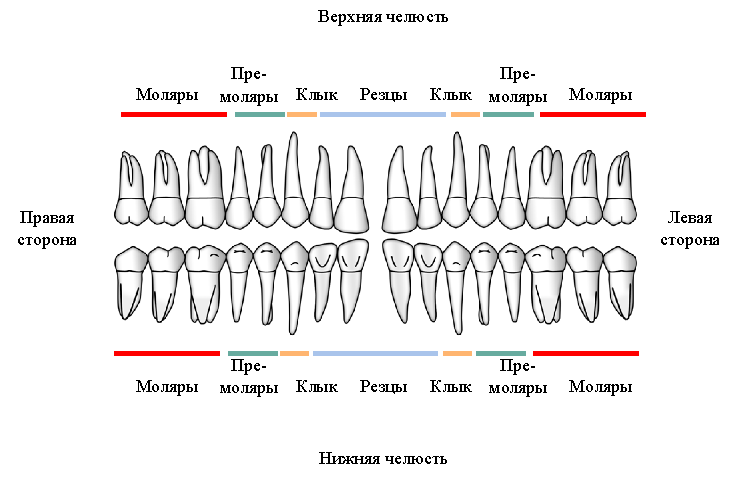
\includegraphics[width=\textwidth]{img/teeth.pdf}
	\caption{Классификация зубов}
	\label{fig:teeth}
\end{figure}

Зубной состав сустава можно представить в виде формулы:

\begin{equation}
	\label{eq:teeth}
	I\frac{2}{2}C\frac{1}{1}P\frac{2}{2}M\frac{3}{3} = 32,
\end{equation}
\eqexplSetIntro{где}
\begin{eqexpl}[15mm]
	\item{$I$} резцы;
	\item{$C$} клыки;
	\item{$P$} премоляры;
	\item{$M$} моляры.
\end{eqexpl}

\subsubsection{Структура вектора особенностей}

Для классификации распознанных зубов можно выделить ряд особенностей, по которым можно определить принадлежность зуба к тому или иному типу.

Среди таких особенностей можно выделить:
\begin{itemize}
	\item размер (площадь в пикселях);
	\item расположение (порядковый номер если считать слева направо);
\end{itemize}

На основе анализа особенностей будет составлена модель, использование которой в машине опорных векторов позволит классифицировать выделенные зубы по типу.

\subsubsection{IDEF0--диаграмма}

На рисунках \ref{fig:idef00} и \ref{fig:idef01} представлена диаграмма IDEF0 метода распознавания.

\begin{figure}[H]
	\centering
	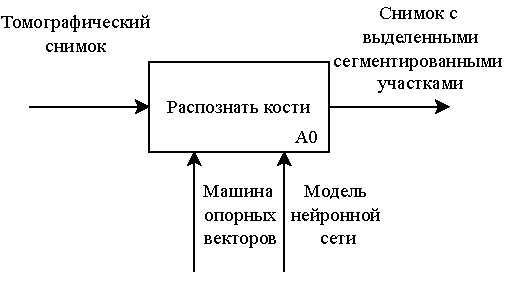
\includegraphics[width=\textwidth]{img/idef00.pdf}
	\caption{IDEF0--диаграмма уровня A0}
	\label{fig:idef00}
\end{figure}

\begin{figure}[H]
	\centering
	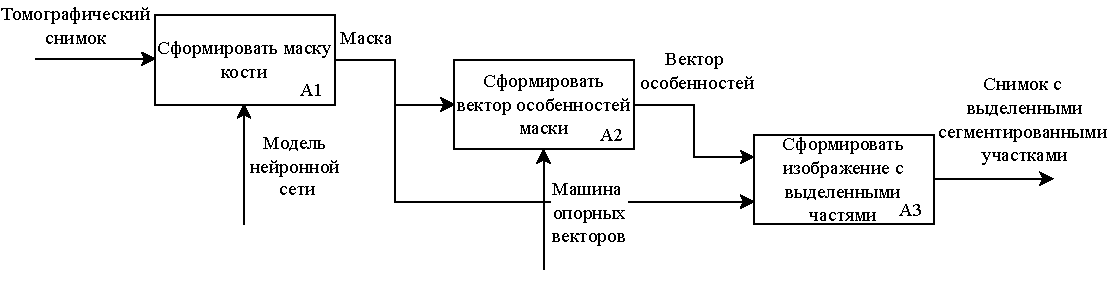
\includegraphics[width=\textwidth]{img/idef01.pdf}
	\caption{IDEF0--диаграмма уровня A1}
	\label{fig:idef01}
\end{figure}

\subsection{Структура разрабатываемого программного комплекса}

Программный комплекс состоит из двух модулей:
\begin{itemize}
	\item Модуль, реализующий модель UNet сети для семантической сегментации;
	\item Пользовательское приложение, производящее сегментацию на основе полученной модели и машины опорных векторов.
\end{itemize}

\subsubsection{Модуль UNet модели}

На рисунке \ref{fig:appunet} представлена схема работы с модулем UNet модели.

\begin{figure}[H]
	\centering
	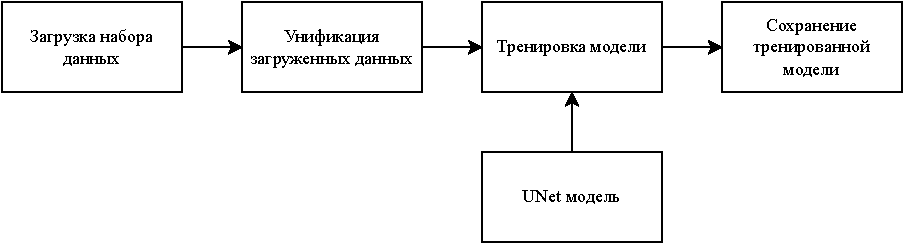
\includegraphics[width=\textwidth]{img/appunet.pdf}
	\caption{Схема работы с модулем UNet модели}
	\label{fig:appunet}
\end{figure}

В данном модуле происходит только тренировка и сохранения модели. Модуль должен быть использован только один раз при первой тренировке модели или когда в модель требуется внести изменения. Вся последующая работа с моделью ведется через файл, который содержит в себе натренированную модель, так как процесс тренировки занимает продолжительное время.

\subsubsection{Модуль пользовательского приложения}

На рисунке \ref{fig:appuser} представлена схема работы с модулем UNet модели.

\begin{figure}[H]
	\centering
	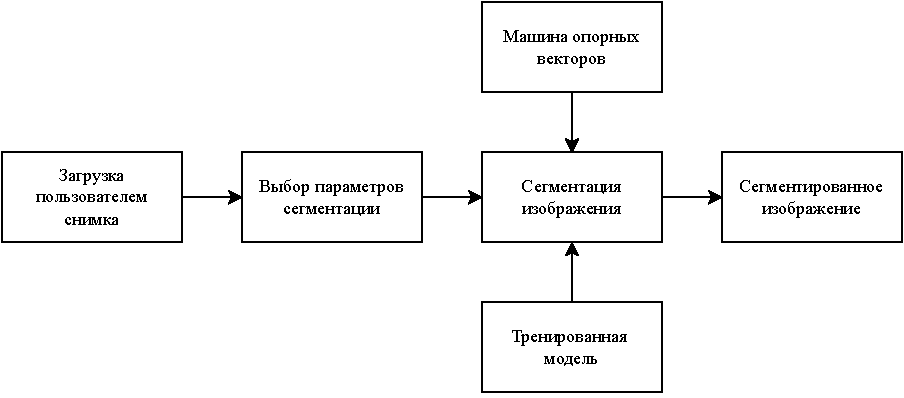
\includegraphics[width=\textwidth]{img/appuser.pdf}
	\caption{Схема работы с модулем пользовательского приложения}
	\label{fig:appuser}
\end{figure}

При работе с данным модулем пользователь может загрузить изображение для дальнейшего анализа и выбрать какие функции нужно применить в процессе распознавания (только выделение костей или также классификация зубов). Результатом работы данного модуля будет являться изображение с выделенными (и классифицированными, при необходимости) костями лица.

\subsection{Данные для обучения модели}

В качестве данных для обучения модели был выбран датасет, состоящий из КТ снимков 116 взрослых пациентов \cite{dataset}. В состав датасета входят снимки как полностью здоровых зубочелюстных суставов, так и суставов с полностью отсутствующим зубным составом. Все снимки сделаны анфас.

На рисунке \ref{fig:example} и \ref{fig:example_teethless} представлены пример КТ снимков из используемого датасета с полностью здоровым зубным составом и с отсутствующим соответственно.

\begin{figure}[H]
	\centering
	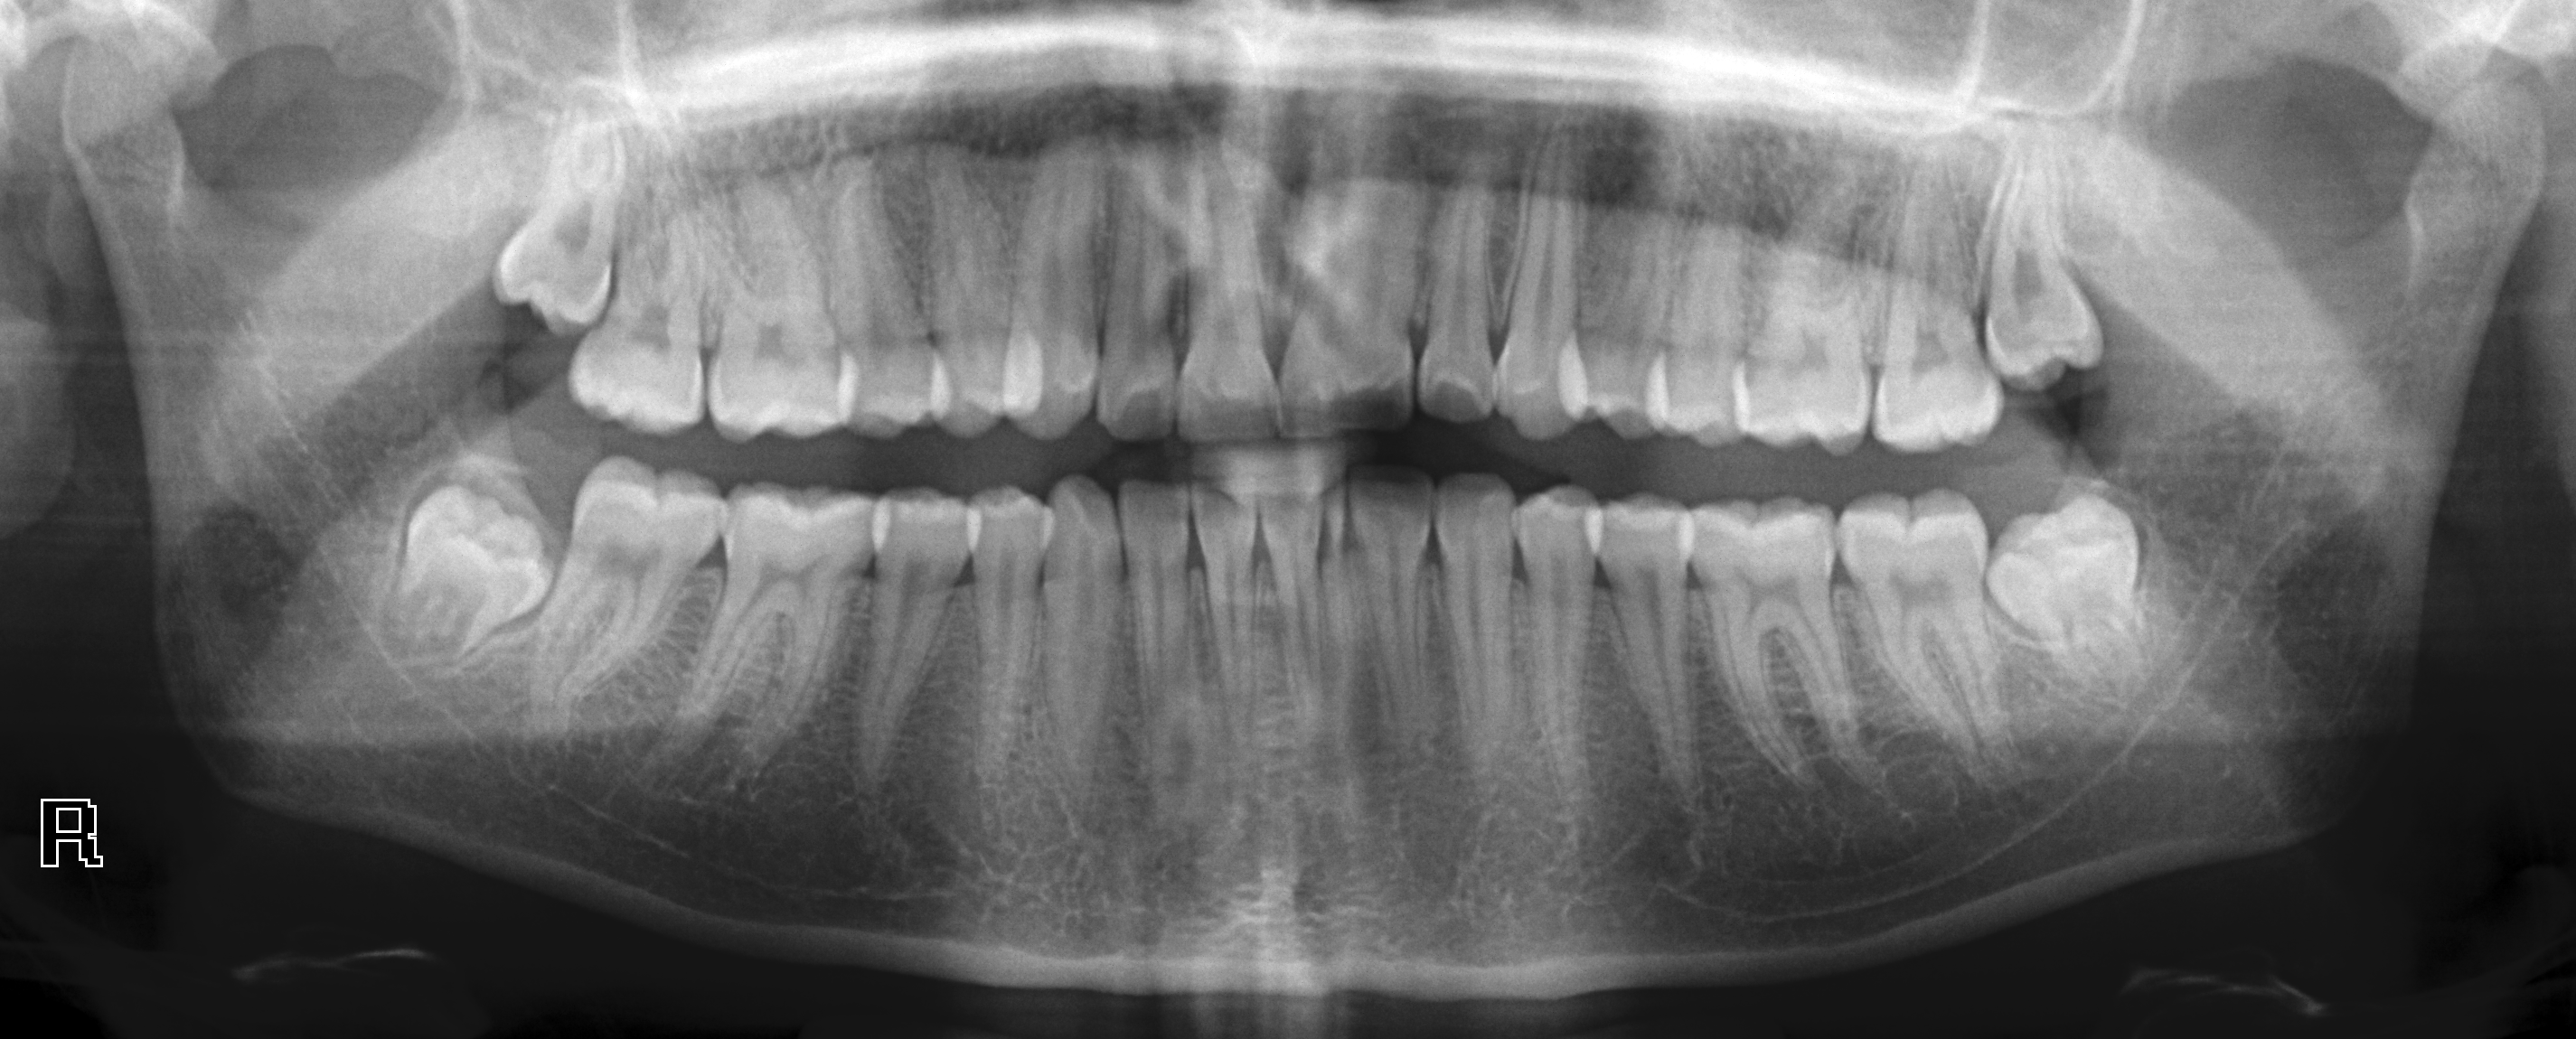
\includegraphics[width=\textwidth]{img/example.png}
	\caption{Пример снимка из датасета (полный зубной состав)}
	\label{fig:example}
\end{figure}

\begin{figure}[H]
	\centering
	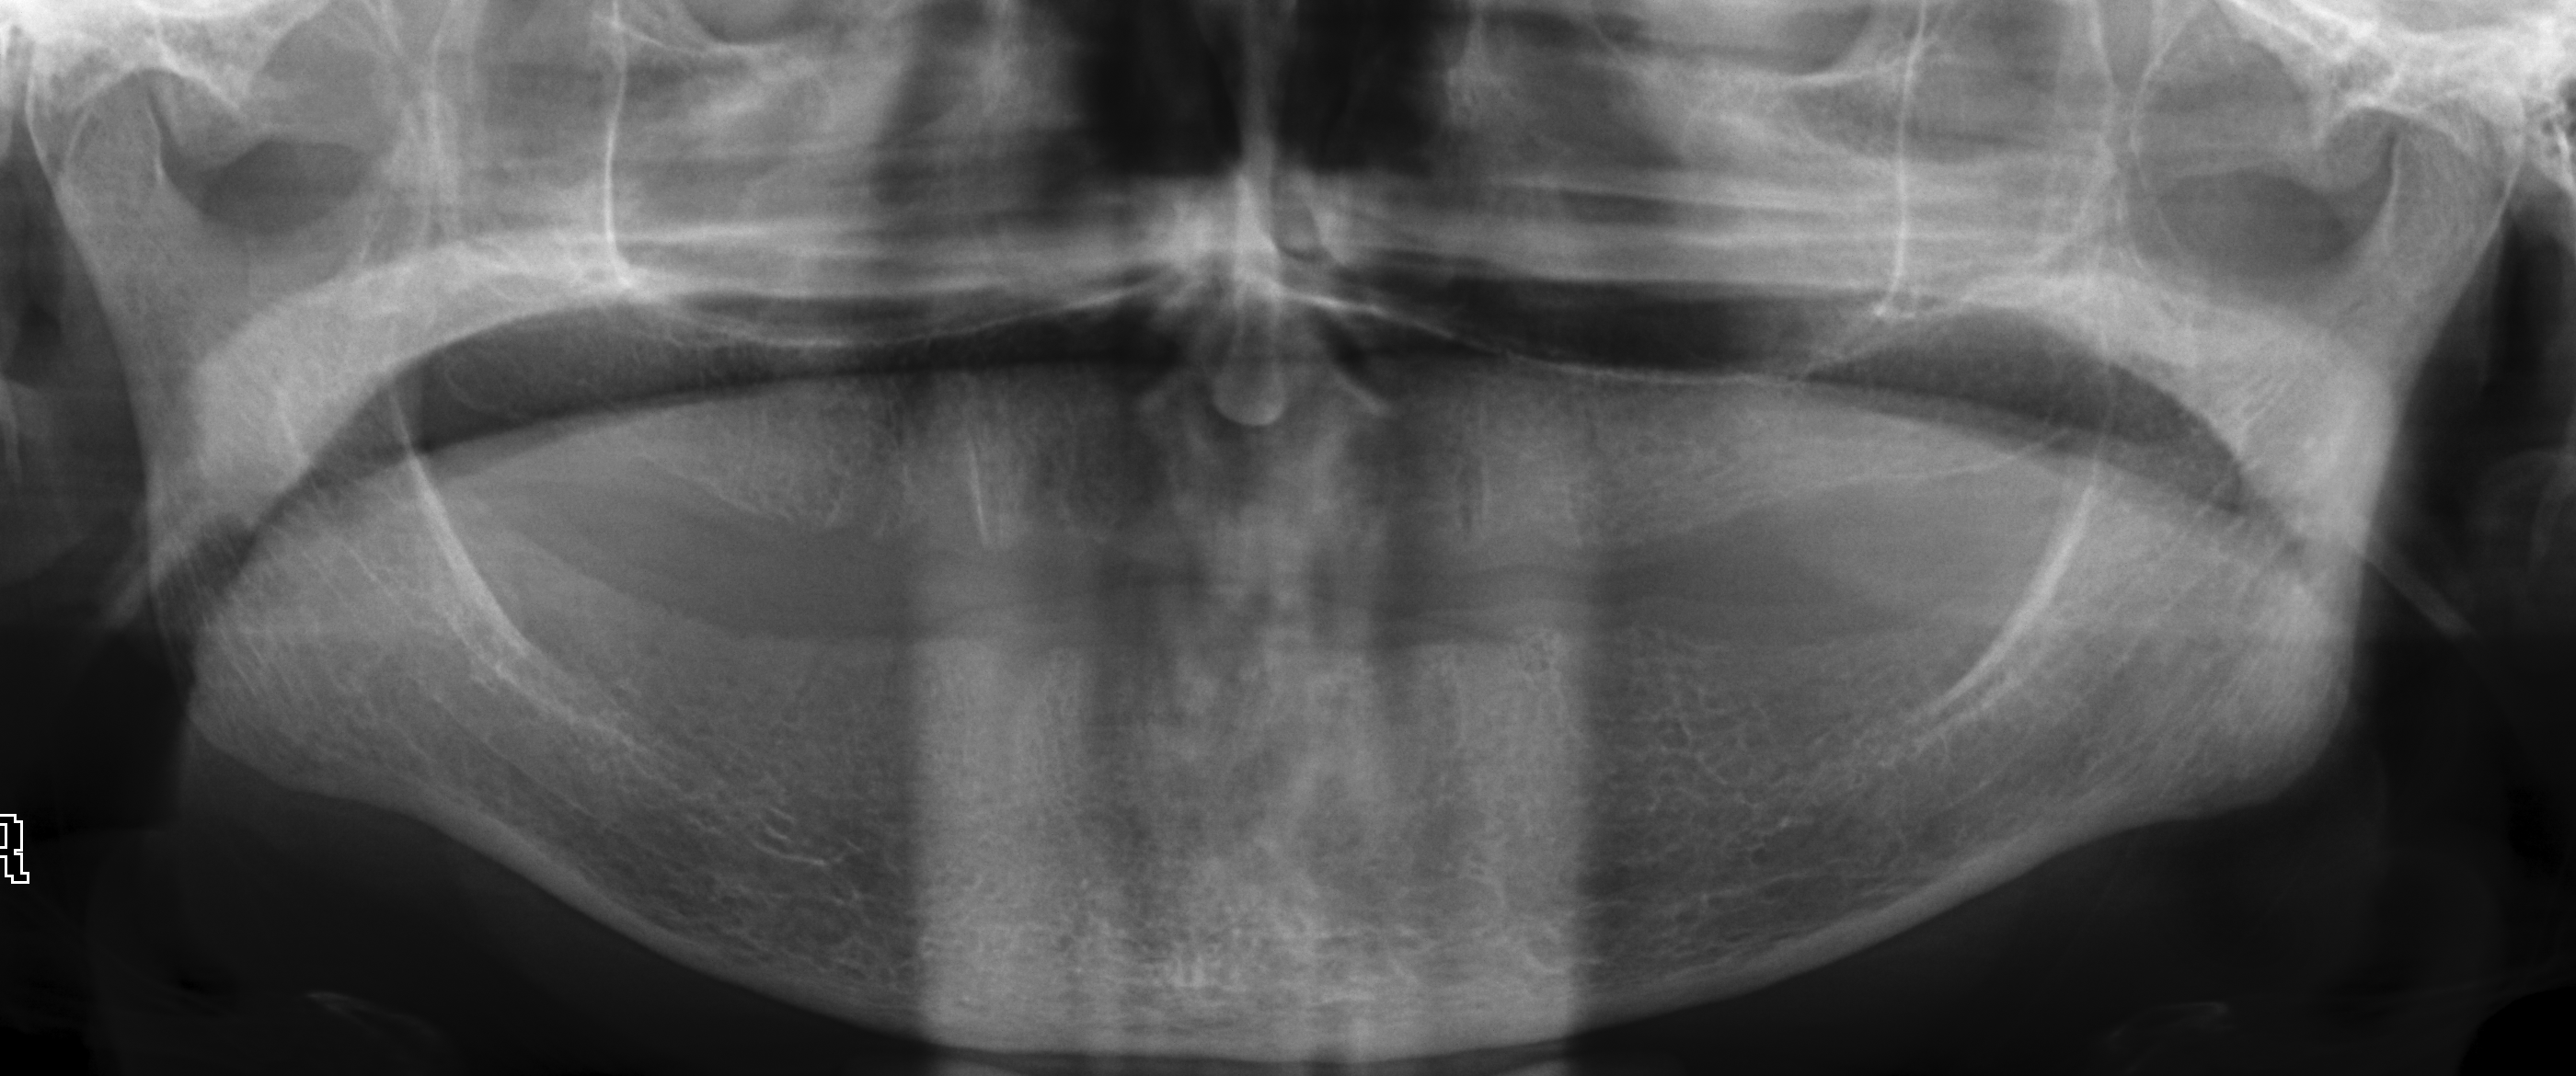
\includegraphics[width=\textwidth]{img/example_teethless.png}
	\caption{Пример снимка из датасета (отсутствующий зубной состав)}
	\label{fig:example_teethless}
\end{figure}

Данные размечены ортодонтами клиники, предоставившей данный датасет. Для каждого снимка размечены нижняя челюсть и зубной состав.

На рисунке \ref{fig:example_mandible} представлен пример разметки нижней челюсти.

\begin{figure}[H]
	\centering
	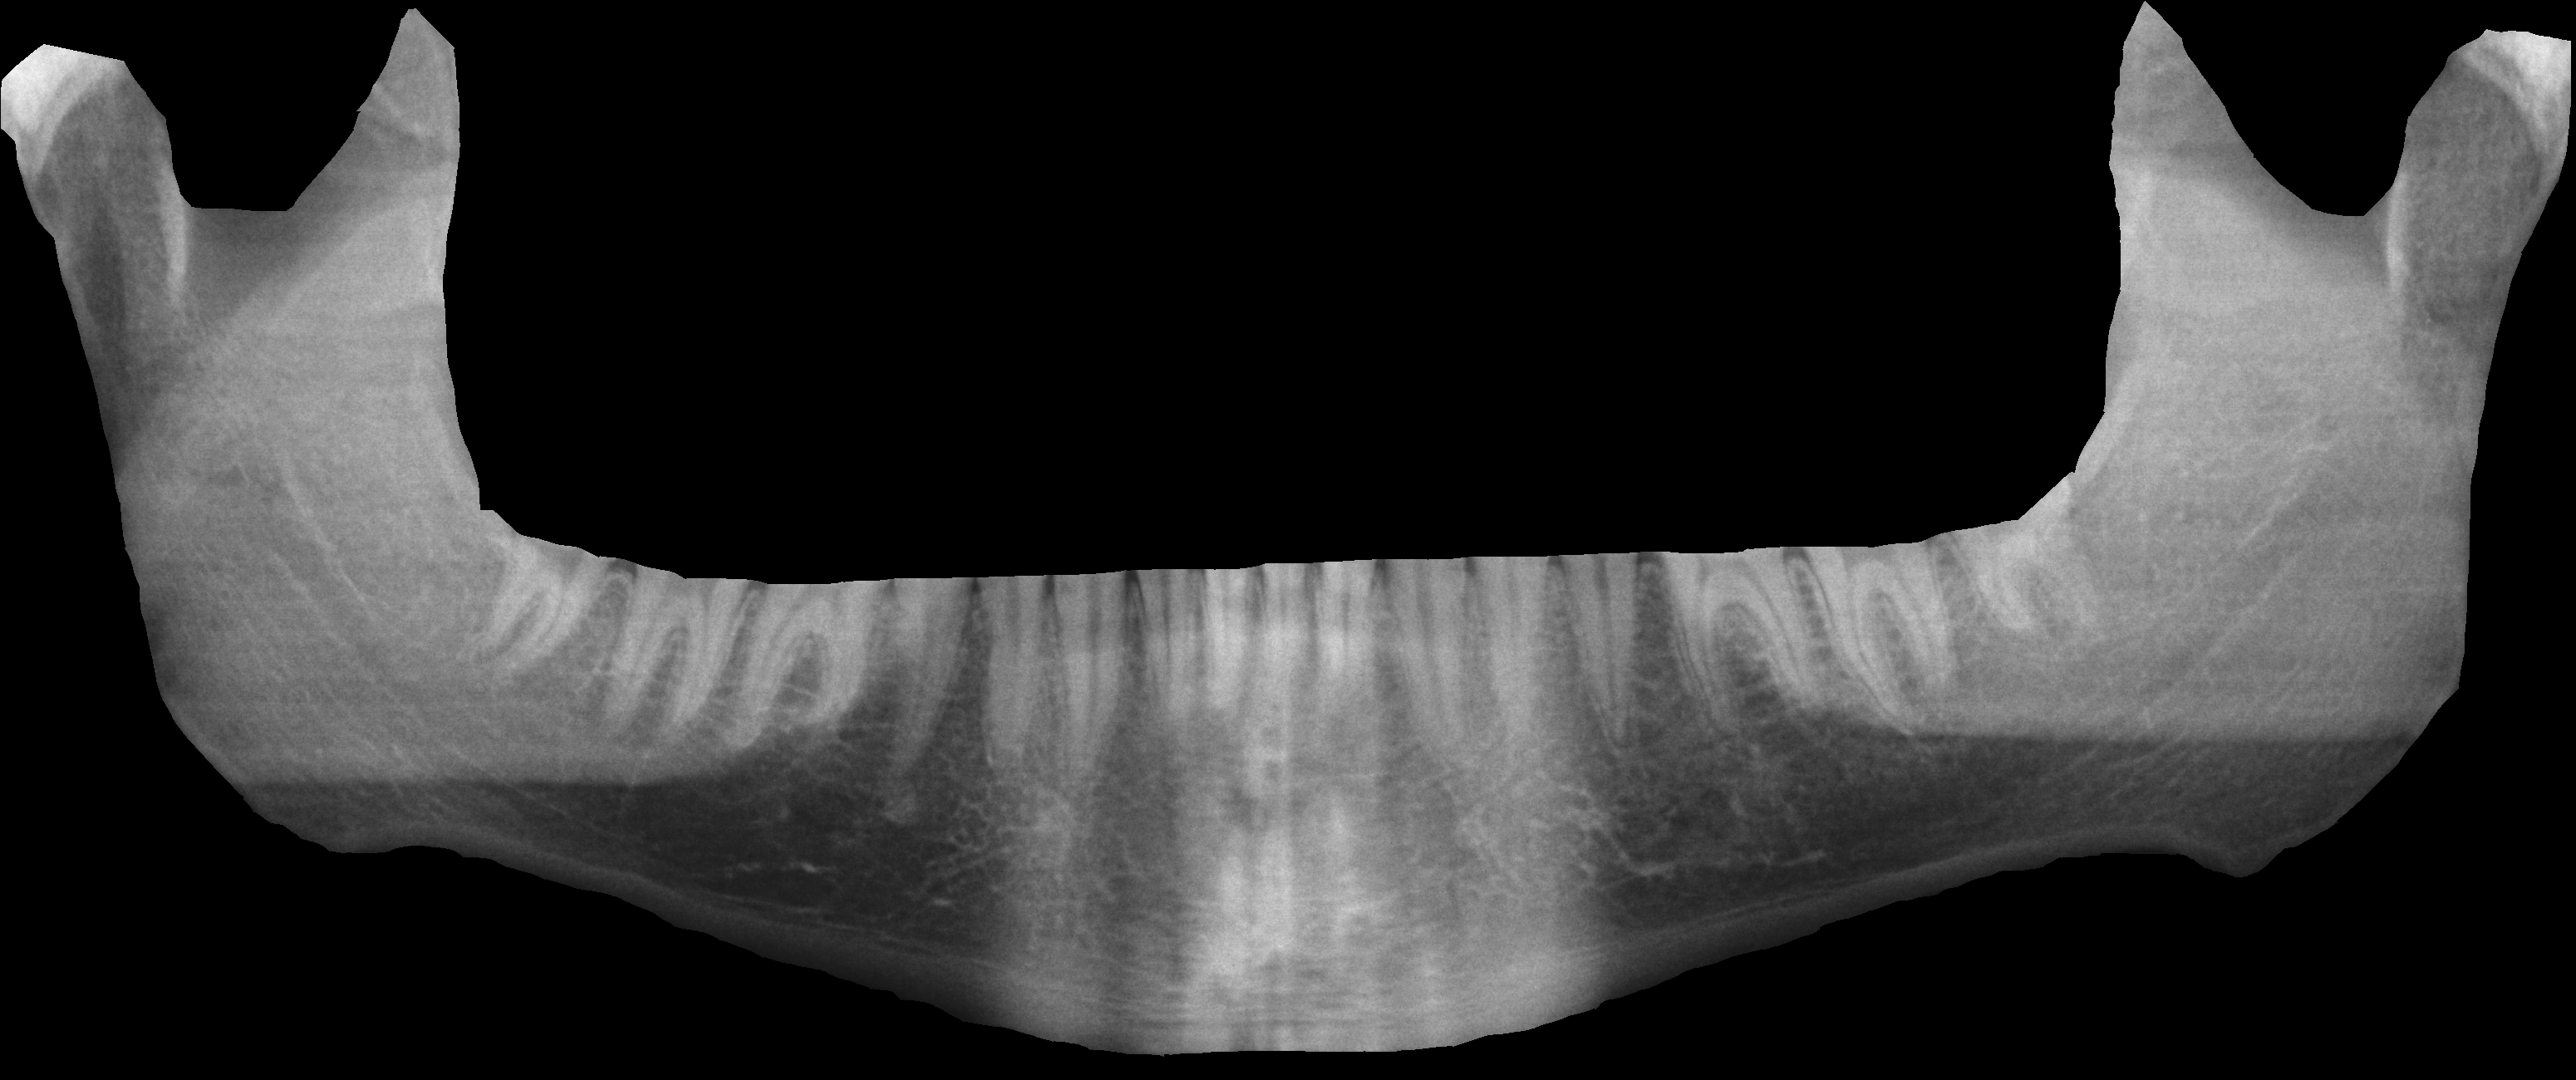
\includegraphics[width=\textwidth]{img/example_mandible.png}
	\caption{Пример разметки нижней челюсти}
	\label{fig:example_mandible}
\end{figure}

\subsection*{Вывод}

Были представлены требования к разрабатываемому методу распознавания и программному комплексу, реализующему интерфейс взаимодействия с методом.

Обозначены особенности разрабатываемого программного комплекса, показано применение машины опорных векторов при классификации распознанных костей.

Представлены схемы работы с разрабатываемыми программными модулями.

Представлен выбор датасета для обучения модели и примеры из него.